\todo{Opisać zgrubnie jak przetwarzany będzie obraz, w celu wykrycia logo \bk. Przygotować schemat blokowy rozwiązania.}

Ogólnie w~algorytmie można wydzielić pięć odrębnych faz przetwarzania. Poszczególne fazy zostały zaprezentowane za pomocą schematu blokowego na rysunku~\ref{fig:algorithm-overview}.

\begin{figure}
    \centering
    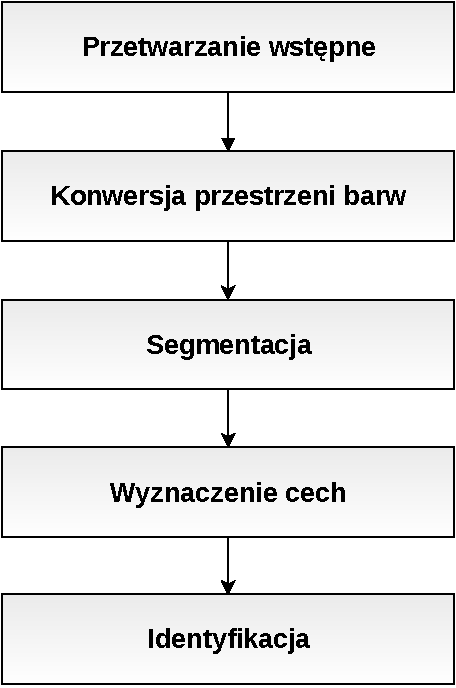
\includegraphics[width=0.6\columnwidth]{figures/algorithmOverview.pdf}
    \caption{Ogólny schemat blokowy algorytmu wykrywania logo \bk}
    \label{fig:algorithm-overview}
\end{figure}